\documentclass[tikz, border=20pt]{standalone}

\usepackage{amsmath, amssymb}
\usetikzlibrary{matrix, positioning, arrows.meta, calc, fit, backgrounds, decorations.pathreplacing}

\pgfdeclarelayer{back}
\pgfdeclarelayer{middle}
\pgfsetlayers{back, middle, main}

\begin{document}
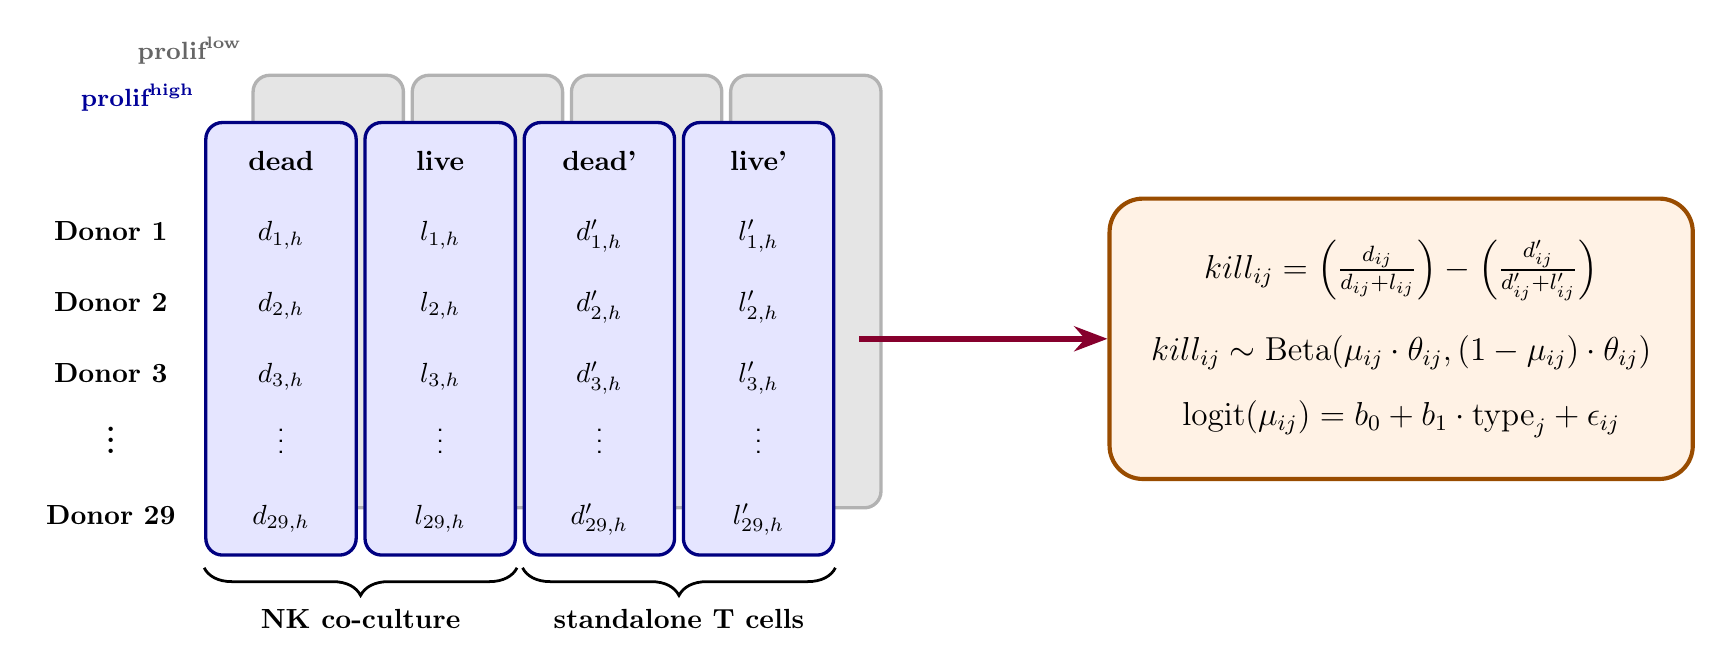
\begin{tikzpicture}[
    font=\sffamily, >=Stealth, thick,
    base_box/.style ={rounded corners=6pt, inner sep=4pt, line width=1.2pt},
    col_front/.style={base_box, draw=blue!50!black, fill=blue!10},
    col_back/.style ={base_box, draw=gray!60, fill=gray!20},
    formula/.style  ={draw=orange!60!black, fill=orange!10, rounded corners=12pt, inner sep=15pt, align=center, line width=1.5pt, font=\large},
    brace_btm/.style={decorate, decoration={brace, amplitude=10pt, raise=4pt, mirror}, line width=1pt},
    zshift/.style   ={xshift=0.6cm, yshift=0.6cm}
]

% Experiment matrix
\matrix (M) [
    matrix of nodes, nodes in empty cells,
    column sep=12pt, row sep=6pt,
    nodes={anchor=center, text height=2.2ex, text depth=0.8ex},
    column 1/.style={anchor=east, font=\bfseries},
    row 1/.style={font=\bfseries},
    cw/.style={nodes={minimum width=1.6cm}},
    column 2/.style=cw, column 3/.style=cw, column 4/.style=cw, column 5/.style=cw
] {
             & dead       & live       & dead'       & live'       \\
    Donor 1  & $d_{1,h}$  & $l_{1,h}$  & $d'_{1,h}$  & $l'_{1,h}$  \\
    Donor 2  & $d_{2,h}$  & $l_{2,h}$  & $d'_{2,h}$  & $l'_{2,h}$  \\
    Donor 3  & $d_{3,h}$  & $l_{3,h}$  & $d'_{3,h}$  & $l'_{3,h}$  \\
    $\vdots$ & $\vdots$   & $\vdots$   & $\vdots$    & $\vdots$    \\
    Donor 29 & $d_{29,h}$ & $l_{29,h}$ & $d'_{29,h}$ & $l'_{29,h}$ \\
};

% Background layer (prolif low)
\begin{pgfonlayer}{back}
    \node[col_back, fit=(M-1-2)(M-6-2), zshift] (col_dead_back) {};
    \node[col_back, fit=(M-1-3)(M-6-3), zshift] (col_live_back) {};
    \node[col_back, fit=(M-1-4)(M-6-4), zshift] (col_dead_sp_back) {};
    \node[col_back, fit=(M-1-5)(M-6-5), zshift] (col_live_sp_back) {};
    \node[anchor=south east, font=\bfseries\small, color=gray!80!black] 
        at (col_dead_back.north west) {prolif\textsuperscript{low}};
\end{pgfonlayer}

% Middle layer (prolif high)
\begin{pgfonlayer}{middle}
    \node[col_front, fit=(M-1-2)(M-6-2)] (col_dead) {};
    \node[col_front, fit=(M-1-3)(M-6-3)] (col_live) {};
    \node[col_front, fit=(M-1-4)(M-6-4)] (col_dead_sp) {};
    \node[col_front, fit=(M-1-5)(M-6-5)] (col_live_sp) {};
    \node[anchor=south east, font=\bfseries\small, color=blue!60!black] 
        at (col_dead.north west) {prolif\textsuperscript{high}};
\end{pgfonlayer}

% Braces
\draw[brace_btm] (col_dead.south west) -- (col_live.south east)
    node[midway, below=15pt, font=\bfseries] {NK co-culture};
\draw[brace_btm] (col_dead_sp.south west) -- (col_live_sp.south east)
    node[midway, below=15pt, font=\bfseries] {standalone T cells};

% Beta regression
\node (eqn) [formula, right=3.5cm of M] {
    $kill_{ij} = \left(\frac{d_{ij}}{d_{ij} + l_{ij}}\right) - \left(\frac{d'_{ij}}{d'_{ij} + l'_{ij}}\right)$ \\[1em]
    $kill_{ij} \sim \text{Beta}(\mu_{ij} \cdot \theta_{ij}, (1-\mu_{ij}) \cdot \theta_{ij})$ \\[0.8em]
    $\text{logit}(\mu_{ij}) = b_0 + b_1 \cdot \text{type}_j + \epsilon_{ij}$
};

% Arrow
\coordinate (arrow_start) at ($(col_live_sp.east)!0.5!(col_live_sp_back.east)$);
\draw[->, line width=2pt, color=purple!70!black] (arrow_start |- eqn.west) -- (eqn.west);

\end{tikzpicture}
\end{document}
